\section{Defining Runtime Enforced Synchronous Neural Networks}
\subsection{\ac{VDTA}: Defining Safety Policies for \ac{CPS}}

\ignore{
We consider our industrial \ac{CPS} systems to have finite ordered sets of input values ${I} = \{{i_1}, {i_2}, \ldots {i_n}\}$ and output values ${O} = \{{o_1}, {o_2}, \ldots {o_n}\}$, where input and output values ${i_n}$ and ${o_n}$ are typed finite binary values.
However, for the purpose of the \ac{AV} case study used in this chapter, the input and output values ${i_n}$ and ${o_n}$ are fixed-point values, taking the form of 32-bit signed integer values.
The input alphabet is ${\Sigma_I} = 32^{{I}}$, i.e. the set made of all possible input value sets; and the output alphabet ${\Sigma_O} = 32^{{O}}$ is likewise the set made of all possible output value sets.
Finally, the input-output alphabet ${\Sigma} = {\Sigma_I} \times {\Sigma_O}$. 
Each input and output event is denoted as a complete set of values, and an input-output event or reaction is of the form $({x_i}, {y_i})$, where ${x_i} \in {\Sigma_I}$ and ${y_i} \in {\Sigma_O}$. 

\begin{example}
	\label{ex:io}
	Within our \ac{AV} braking example, using the \ac{VDTA} defined by the $\mathcal{V}_{ped}$ safety policy represented by Figure~\ref{fig:avpedrte}, let ${I} = \{{O_2}, {O_5}, {O_{2_v}}, {O_{5_v}}, {S}\}$ which are 32-bit signed integers representing objects 2 and 5 in the system, their velocities and the speed of the vehicle respectively.
	Then, let the output ${O} = \{{D}\} = \{{\langle A, B_S, B_H \rangle}\}$, where ${D}$ is a vector of signed 32-bit integers, representing the \textit{decision} (action) taken by the vehicle this tick (\textit{Accelerate}, \textit{Soft Brake} and \textit{Hard Brake}).
	
	Then the input-output event ${O_2}=65536$, ${O_5}=0$, ${O_{2_v}} = 655360$, ${O_{5_v}} = 0$,  ${S} = 4063232$, ${D} = \langle 0, 0, 65536 \rangle$ is denoted as:\\$(\{65536, 0, 655360, 0, 4063232\}, \{\langle 0, 0, 65536 \rangle\})$ where each value is a fixed-point (32-bit signed integer) representation of a floating point value, i.e. Object 2 is a pedestrian, Object 5 is nothing, Object 2 is travelling at 10 km/h, Object 5 is not moving, and the vehicle's speed is 62 km/h, while the decided action for this tick is hard braking ($B_H$).
\end{example}
}



We consider our industrial \ac{CPS} systems to have finite ordered sets of valued input channels ${I} = \{{i_1}, {i_2}, \ldots {i_n}\}$ and valued output channels ${O} = \{{o_1}, {o_2}, \ldots {o_n}\}$.



A VDTA can be seen as a DTA with finite set of locations, and a finite set of discrete clocks used to represent time evolution, extended with internal variables and external input (resp. output channels) called as external variables used for representing system data.
In a VDTA, a transition consists of an action carrying values of external variables, a guard on internal variables, external variables and clocks, and an assignment of internal variables, and reset of clocks.
In a VDTA, internal variables are used for internal computation, and
external variables model the data carried by the actions from the monitored system (resp. environment). 
%Thus, each input (resp. output channel) is considered as an external variable. 

%
For a variable (resp. channel) $v$, ${\cal D}_v$ denotes its domain,
and for a tuple of variables $V= (v_1, \ldots, v_n)$,
${\cal D}_V$ is the product domain ${\cal D}_{v_1} \times \cdots \times {\cal D}_{v_n}$.
%A predicate $P(V)$ on a tuple of variables $V$ is a logical formula whose semantics is a function ${\cal D}_V \rightarrow \{\true, \false\}$.
A valuation of the variables in $V$
is a mapping $\nu$ which maps every variable $v \in V$ to a value $\nu(v)$ in ${\cal D}_v$.
%
Let $X=\{x_1,\ldots, x_k\}$ be a finite set of integer variables (i.e., discrete clocks).
%
A {\em valuation} for $x$ is an element of $\bbn$, that is a function from $x$ to $\bbn$.
The set of valuations for the set of clocks $X$ is denoted by $\chi$.
%
For $\chi\in\bbn^V$, $\chi+1$ is the valuation assigning $\chi(x)+1$ to each clock variable $x$ of $X$.
Given a set of clock variables $X' \subseteq X$, $\chi[X' \leftarrow 0]$ is the valuation of clock variables $\chi$ where all the clock variables in $X'$ are assigned to $0$.

Monitors input and output words. A word is a sequence $\sigma = e_1\cdot e_2 \cdots e_n$ where $\forall i \in [1,n]: e_i = a_i(\eta_i)$ where $a_i \in \Sigma$ is an action and $\eta_i \in {\cal D}_V$ is a vector of values of a tuple of variables $V$. 


%
\begin{definition}[Syntax of {VDTA}s]
	\label{def:vdta}
	A {VDTA} is a tuple \\
	$\calA = \left(\Sigma, L, {l_0}, X, V, C, \Theta, F,  \Delta \right)$ where:
	\squishlist
	\item $\Sigma$ is a non-empty finite set of actions,
	and an action $a \in \Sigma$ has a signature $sig(a) = ( t_0, t_1, \ldots, t_k )$ which is a tuple of types of the external variables,
	\item $L$ is a finite non-empty set of locations, with $l_0 \in L$ the initial location, and $F \subseteq L$ the set of accepting locations;
	\item $X$ is a finite set of discrete clocks;
	\item $V$ is a tuple of typed internal variables \item $C$ is a tuple of external variables, where $C = I \cup O$, where $I$ is the set of input channels, and $O$ is the set of output channels; 
	\item $\Theta\subseteq {\cal D}_{V }$ the initial condition, is a computable predicate over $V$;
	\item $\Delta$ is a finite set of transitions, and each transition $t \in \Delta$ is a tuple $( l, a, c, G, A, l' )$
	also written\\
	$l \xrightarrow{a(c), G(V,c), V':=A(V,c)} l'$
	such that,
	\squishlist
	\item[\textbullet] $l, l' \in L$ are respectively the origin and target locations of the transition;
	\item[\textbullet] $a \in \Sigma$ is the action, and $c=( c_1, \ldots c_k )$ is a tuple of external variables local to the transition;
	\item[\textbullet] $G = G^D \wedge G^X$ is the guard where
	\squishlist
	\item[-] $G^D \subseteq {\cal D}_V \times {\cal D}_{sig(a)}$
	is a computable predicate over internal variables and external variables  in $V \cup c$;
	\item[-] $G^X$ is a clock constraint over $X$ defined as a Boolean combinations of constraints of the form $x \sharp f(V \cup c)$, where $x \in X$ and $f(V \cup c)$ is a computable function, and $\sharp \in \{ <, \leq, =, \geq, > \}$;
	\squishend
	\item[\textbullet] $A$$=$$(A^D, A^X)$ is the assignment of the transition where
	\squishlist
	\item[-] $A^D :{\cal D}_V \times {\cal D}_{sig(a)} \rightarrow {\cal D}_V$ defines the evolution of internal variables.
	\item[-] $A^X \subseteq X$ is the set of clocks to be reset.
	\squishend
	\squishend
	\squishend
\end{definition}
%

\begin{example}
	The case study can be presented by four, different \acp{VDTA}; $\mathcal{V}_{ped}$, $\mathcal{V}_{car}$, $\mathcal{V}_{drive}$ and $\mathcal{V}_{cnn}$, as depicted in Figures~\ref{fig:avpedrte}, \ref{fig:avcarrte}, \ref{fig:avdriverte} and \ref{fig:avcnnrte} respectively. 
	For the purposes of these examples, the \ac{VDTA} for the pedestrian safety policy, $\mathcal{V}_{ped}$, is used.
	This \ac{VDTA} specifies that driving into a pedestrian in-front (if any) and not braking hard is a violation, and approaching a pedestrian from a distance (if any) and not starting to slow down (braking softly) is a violation.
	
	This is encoded as a \ac{VDTA} with a set of locations $L = \{l_{drive}, l_{brake}, l_v\}$ and accepting locations $F = \{l_{drive}\}$, with the initial state being $l_{drive}$.
	The set of external variables $C = \{O_2, O_5, O_{2_v}, O_{5_v}, S, A, B_S, B_H\}$ are all 32-bit signed integers, where $O_2$, $O_5$, $O_{2_v}$, $O_{5_v}$ and $S$ are input channels and $A$, $B_S$ and $B_H$ are output channels.
	The set of actions $\Sigma = \{tk(O_2, O_5, O_{2_v}, O_{5_v}, S, A, B_S, B_H)\}$, and the set of internal variables $V = \{T_{lim}\}$, where $T_{lim}$ is a 32-bit signed integer.
	In the example, $\tau$ is a function with $O_2$, $O_5$, $O_{2_v}$, $O_{5_v}$ and $S$ as input parameters. 
	
	In this \ac{VDTA} there are two violation transitions, labelled \textcircled{a} and \textcircled{b} in Figure~\ref{fig:avpedrte}.
	\textcircled{a} occurs when the vehicle does anything else other than braking when there is a pedestrian in-front or not braking when there is no pedestrian ahead of the vehicle.
	\textcircled{b} can also occur when the vehicle has not braked enough within a certain period of time $T_{lim}$, or when the vehicle remains braking longer than is safe or necessary.
	This represents the vehicle taking further unsafe actions when already in an unsafe state.
\end{example}

Policy \ac{VDTA} are required to be \textit{deterministic}, i.e. for any given state, the conjunction of any guards of any other outgoing transitions may not be satisfiable; and \textit{complete}, i.e. for any given state at any given time and any given event, at least one transition guard is satisfied.

\subsection{Semantics for \ac{VDTA}}

Let $\calA = \left(\Sigma, L, {l_0}, X, V, C, \Theta, F,  \Delta \right)$  be a VDTA.
The semantics of $\calA$ is a timed transition system,
where a state consists of a location, and valuations of internal variables $V$ and clocks $X$, and actions associated with values of external variables in $C$.

\begin{definition}[Semantics of {VDTA}s]
	\label{def:vdta:semantics}
	The semantics of $\calA$ is a timed transition system $\sem{\calA}=( Q, q_0, Q_F, \Gamma, \to )$, defined as follows:
	\squishlist
	\item $Q = L \times {\cal D}_V \times \bbn^V$, is the set of states of the form $q= ( l,\nu ,\chi )$ where
	$l \in L$ is a location,
	$\nu \in {\cal D}_V$ is a valuation of internal variables,
	$\chi$ is a valuation of clocks;
	\item $Q_0 = \{ ( l_0,\nu, \chi_{[X \leftarrow 0]} )  \mid \Theta(\nu)=\true \}$ is the set of initial states;
	\item $Q_F = F \times {\cal D}_V \times \bbn^V$ is the set of accepting states;
	\item $\Gamma = \{ a(\eta) \mid
	a \in \Sigma \wedge \eta \in {\cal D}_{sig(a)}  \}$ is the set of transition labels;
	\item $\to\subseteq Q\times \Gamma\times Q$  the transition relation
	is the smallest set of transitions of the form
	$( l,\nu,\chi \rangle \longrightarrow {a(\eta)} \langle l',\nu',\chi')$
	such that  $\exists ( l, a, c, G, A, l' ) \in \Delta$,
	with $G^X(\chi + 1) \wedge G^D(\nu, \eta) $ evaluating to {\true},
	$\nu'= A^D(\nu, \eta)$ and $\chi'=(\chi+1)[A^X \leftarrow 0]$.
	\squishend
\end{definition}


%The set of timed words over $\Sigma$ where the actions carry parameter value and other data is denoted by $\tw(\Lambda)$.
A {\em run} $\rho$ of $\sem{\calA}$ from a state $q\in Q$ over a {\em trace} $w =  a_1(\eta_1)\cdot a_2(\eta_2)\cdots a_n(\eta_n)$ is a sequence of moves in $\sem{\calA}$:
$\rho = q \xrightarrow {a_1(\eta_1)} q_1
\cdots q_{n-1}\xrightarrow {a_n(\eta_n)} q_{n}$,
for some $n\in\bbn$.
The set of runs from the initial state $q_0\in Q$,  is denoted $\Run(\calA)$ and $\Run_{Q_F}(\calA)$ denotes the subset of those runs {\em accepted} by $\calA$, i.e.,  ending in an accepting state $q_n \in Q_F$.

%%%%%%%%%%%%%%%%%%%%%%%%%%%%%%%%%%%%%%%%%%%%%%%
%%%%%%%%%%%%%%%%%%%%%%%%%%%%%%%%%%%%%%%%%%%%%%%
\ignore{
\begin{example}[Run of a VDTA]
	Let us consider the VDTA discussed in Example\ref{eg:vdta} presented in Figure\ref{fig:vsa-overcurrent}. 
	An example run of the VDTA presented in Figure~\ref{fig:vsa-overcurrent} is presented here.
	Let the internal variable $i_{max}$ be initialized with 10000.
	A run of this VDTA starting from the initial state $(l_{safe}, i_{max}=10000, x = 0)$ for the word $\sigma = tk(4000, 5000,1)\cdot tk(8000, 5000,1)\cdot tk(7000, 5000,1)\cdot tk(8000, 5000,1)\cdot tk(8000, 5000,1)\cdot tk(8000, 5000,1)$ is given below:\\
	
	$(l_{safe}, i_{max}=10000, x = 0)\xrightarrow {tk(4000, 5000,1)} (l_{safe}, i_{max}=10000, x = 1)
	\xrightarrow {tk(8000, 5000,1)}
	(l_{unsafe}, i_{max}=10000, x = 0)
	\xrightarrow { tk(7000, 5000,1)}
	(l_{unsafe}, i_{max}=10000, x = 1)
	\xrightarrow { tk(8000, 5000,1)}
	(l_{unsafe}, i_{max}=10000, x = 2)
	\xrightarrow { tk(8000, 5000,1)}
	(l_{unsafe}, i_{max}=10000, x = 3)
	\xrightarrow { tk(8000, 5000,1)}
	(l_{vio}, i_{max}=10000, x = 4)
	$
\end{example}
}


\begin{example}[Run of a VDTA]
	\label{ex:run}
	An example run of the VDTA presented in Figure~\ref{fig:avpedrte} is presented here.
	Assume that the time the vehicle has to be braking is $T_{lim} = 2$. 
	The starting state is $l_{drive}$, and the first I/O event is $(\{0, 0, 0, 0, 4063232\}, \{\langle 0, 0, 0 \rangle\})$, i.e. nothing is detected in-front of the vehicle and the vehicle does not accelerate or brake, meaning it is cruising at 62 km/h.
	Thus, the automaton remains in state $l_{drive}$.
	Next tick, $(\{0, 65536, 0, 655360, 4063232\}, \{\langle 0, 65536, 0 \rangle\})$ occurs, i.e. a pedestrian is detected quite far ahead of the vehicle, moving across the road at 10 km/h, and the vehicle is taking a soft braking action from 62 km/h.
	Since ${O} = \{\langle 0, 65536, 0 \rangle\}$ which is a soft brake $B_S$ and Object 5, far ahead of the vehicle, is a pedestrian $O_5 = 65536 = O_{5_P}$ the system enters the unsafe state $l_{brake}$ and $t = 0$ is set.
	Then,  $(\{65536, 0, 0, 0, 2621440\}, \{\langle 0, 0, 0 \rangle\})$ is received, i.e. the pedestrian has stopped moving in the road and is now close to the vehicle, however the vehicle is not braking, but rather cruising at 40 km/h.
	Since no braking is detected, the violation transition $l_v$ is taken.
	As such, this run was \textit{non-accepting}.
\end{example}

\subsection{Defining Safety Automata for an \ac{AV} system}
In order for the \ac{AV} system to operate safely, it must follow a set of policies ($\mathcal{V}$), defined in English here:

$\mathcal{V}_{cnn}$: The output of the vision \ac{CNN} ensemble networks ($O$) must match the \ac{LiDAR} values ($L$) when the confidence of the ensemble networks is low. 
If the confidence is high, and there is a mismatch, the output should be classified as \textit{unknown} ($U$).
The system should treat this output as if it were a pedestrian, i.e. with utmost caution.

$\mathcal{V}_{drive}$: The vehicle may not exceed the safe speed limit. 
An \textit{acceleration} command $A$ should be suppressed when the vehicle's speed limit of 100km/h is reached.

$\mathcal{V}_{car}$: Ensure that the car does not drive into other vehicles. If an \textit{acceleration} command $A$ is asserted when the car in front (i.e. $O_{2_C}$ or $O_{5_C}$) is driving slower than the \ac{AV} ($O_{2_V}<S|O_{5_V}<S$), then this is suppressed and instead an appropriate brake speed $B_S$ (soft) or $B_H$ (hard) would be asserted instead.

$\mathcal{V}_{ped}$: Ensure that the car does not behave unsafely around pedestrians. If a pedestrian appears in-front of the vehicle $P=true$, then the car should select an appropriate braking action (either $B_S$ or $B_H$). If a pedestrian remains off to the side of the vehicle, then either the vehicle should cruise or a braking action is appropriate.

We can define these rules of the \ac{AV} system as a \textit{Safety Automata}~\cite{recps}, which are a kind of \acf{DTA}. 
Examples of this are presented in Figures \ref{fig:avpedrte} - \ref{fig:avcnnrte}, which represent the automata used in the four policies of the \ac{AV} system.
%Here, $A$ refers to the accelerate action, $B_S$ refers to a slow, or gentle, braking action, $B_H$ refers to a hard braking action.
$P$ is a flag that denotes the presence of a pedestrian in a position that will be dangerous at any point in the future, and $t$ is a timer that ensures that the \ac{AV} has braked for long enough and in time when a collision with a pedestrian has been detected, denoted by the time $T_{lim}$. 
$T_{lim}$ is a predefined length of time by which the system should have reacted to a pedestrian in a dangerous position.

Finally, a complete policy framework can be established by simply ANDing the component policies together, i.e. \\ $\mathcal{V}_{av} = \mathcal{V}_{cnn} \wedge \mathcal{V}_{drive} \wedge \mathcal{V}_{car} \wedge \mathcal{V}_{ped}$.

\begin{figure}[H]
	\centering
	\includegraphics[width=\linewidth]{avpedrte.tikz}
	\caption{Safety Automaton for Policy $\mathcal{V}_{ped}$\label{fig:avpedrte}}
\end{figure}
\begin{figure}[H]
	\centering
	\includegraphics[width=0.5\linewidth]{avcarrte.tikz}
	\caption{Safety Automaton for Policy $\mathcal{V}_{car}$\label{fig:avcarrte}}
\end{figure}
\begin{figure}[H]
	\centering
	\includegraphics[width=0.5\linewidth]{avdriverte.tikz}
	\caption{Safety Automaton for Policy $\mathcal{V}_{drive}$\label{fig:avdriverte}}
\end{figure}
\begin{figure}[H]
	\centering
	\includegraphics[width=0.5\linewidth]{avcnnrte.tikz}
	\caption{Safety Automaton for Policy $\mathcal{V}_{cnn}$\label{fig:avcnnrte}}
\end{figure}


\subsection{Enforcing Non-accepting I/O Events}
Enforcers are designed to prevent a system from generating an input/output trace that is non-accepting, such as Example~\ref{ex:run}.
\cite{recps} proposed \ac{DTA} semantics with two possible methodologies for editing non-accepting I/O events.
These are \textit{random} and \textit{minimum} edits; a random edit chooses a random, accepting event from a list of accepting I/O events and minimum edit chooses the closest accepting event to the current non-accepting event.
However, neither of these edits are not always useful for problems in real scenarios.
Take Example~\ref{ex:run}, when the transition $l_{drive} \rightarrow l_v$ is taken, Object 2 can be edited such that $l_v$ is not entered, however this will not remove the danger that initially posed this transition.
However, if the action ${O}$ was changed, e.g. the cruising action in the example that caused the non-accepting trace was changed to a hard braking action, then an accepting event would have occurred \textit{and} the pedestrian in the road would have been safe.

In general, then, the designer of any given policy should also select their preferred edit actions out of the list of possible safe edits for each violation transition, thus ensuring practical runtime enforcement.

\begin{example}[Selected Edit Actions for a VDTA]
	In Figure~\ref{fig:avpedrte}, there are many different actions in $\Sigma$ that, when taken in a specific location $L$ result in a violation transition.
	In this example, a situation where the current locations is $l_{drive}$ and the action is $\Sigma = \{tk(1, 0, 10, 0, 30, 1, 0, 0)\}$, i.e. there is a pedestrian directly in front of the vehicle moving at 10 km/h, while the vehicle is moving directly forward at 30 km/h and is accelerating.
	Thus, the violation transition \textcircled{a} occurs.
	\squishlist
	\item Transition \textcircled{a}: $A := 0$, $B_S := 0$ and $B_H := 1$
	\squishend
	The recovery for this violation transition changes the vehicle to not accelerate, but rather brake hard.
	This instead changes the transition to $l_{drive} \rightarrow l_{brake}$, which is a safe transition that slows the vehicle down before it hits the pedestrian.
\end{example}
%The first policy, $\mathcal{V}_{cnn}$, compares the \ac{LiDAR} depiction and the classified image class from the corresponding ensemble outputs, if the \ac{LiDAR} and ensemble outputs are different, and the ensemble confidence value is low, the ensemble output is changed to match the output of the corresponding \ac{LiDAR} reading.
%If the ensemble confidence is high, both the \ac{LiDAR} reading and the corresponding ensemble output are changed to signal that the object detected is \textit{Unknown} and should be treated with extra caution, as if the object were a pedestrian.
%The second policy, $\mathcal{V}_{drive}$, ensures that the vehicle maintains reasonable driving practices on the road, e.g. not staying stationary in the middle of the road and not speeding.
%If the \ac{AV} controller outputs that the \ac{AV} should \textbf{accelerate} while the \ac{AV} is at the speed limit, the \textbf{accelerate} command would be changed to a  \textbf{cruise} command.
%Likewise, if the \ac{AV} controller decides that the \ac{AV} should remain stationary in an empty road, the \textbf{brake} (or \textbf{cruise}) command would be modified to an \textbf{accelerate} command.
%The third policy, $\mathcal{V}_{car}$, checks the environment for other vehicles and ensures that the \ac{AV} does not drive into other vehicles, or cause accidents with other vehicles in any way.
%If the \ac{AV} would \textbf{accelerate} into a vehicle in front, the \textbf{accelerate} would be changed to a \textbf{cruise}, if the \ac{AV} was driving much faster than the vehicle in front and the \ac{AV} is not braking, the current action would be modified to be a \textbf{brake} action.
%The fourth, and highest priority, policy ($\mathcal{V}_{ped}$) monitors the environment for pedestrians and ensures that the car does not exhibit unsafe behaviour with regards to the pedestrians. 
%If the \ac{AV} were to \textbf{accelerate}, or \textbf{cruise}, into a pedestrian that is in front of the vehicle, or approaching the road from the sides, the \textbf{accelerate}, or \textbf{cruise}, action would be changed to a \textbf{brake} action.
%If the \ac{AV} does not brake fast enough with a pedestrian in front of the \ac{AV}, or approaching from the sides, a \textbf{hard brake} action would be initiated instead of the \ac{ANN} proposed action.
%This policy ensures that the vehicle always drives slowly and cautiously around pedestrians.


\subsection{\ac{SANN}: Defining Artificial Neural Networks for \acp{CPS}}
\begin{definition}[Layer of a Synchronous \ac{CNN}]
	\label{def:layer}We define the \emph{\ac{SANN} Layers} as a tuple $\mathcal{L} = (\mathcal{I}, \mathcal{O}, \mathcal{W}, \mathcal{T}, \tau)$:
	\begin{itemize}
		\item $\mathcal{I} = \{i_0, i_1, ..., i_k \}$ are the $k$ inputs to the layer, represented by a vector of 32-bit signed integers.
		\item $\mathcal{O} = \{o_0, o_1, ..., o_k \}$ are the $k$ outputs from the layer, represented by a vector of 32-bit signed integers.
		\item $\mathcal{W} = \{w_0, w_1, ..., w_k\}$ are the $k$ weights associated with the layer, represented by a vector of 32-bit signed integers.
		\item $\mathcal{T}$ is the layer type and determines the operations applied to the weights and inputs, where $\mathcal{T}~\in~\{Dense, Convolutional, Maximum~pool, Average~pool\}$.
		\item $\tau(\mathcal{I}, \mathcal{W}, \mathcal{T}) = \mathcal{O}$ is the non-linear function that produces an output set $\mathcal{O}$ given inputs $\mathcal{I}$, weights $\mathcal{W}$ and layer type $\mathcal{T}$. 
	\end{itemize}
\end{definition}

\begin{definition}[Synchronous \acp{CNN}]
	\label{def:cnn}
	A Synchronous \ac{CNN} is an extension of the previously defined \ac{SANN} from Definition~\ref{def:bb-mlp}. We define a \emph{Synchronous \ac{CNN}} as a tuple $\mathcal{C} = (\mathcal{I}, \mathcal{O}, \mathcal{A}, \eta)$ where
	\begin{itemize}
		\item $\mathcal{I}$ is a finite collection of 32-bit signed integer input variables with the domain \textbf{I}$ = 32^n$, where $n$ is the number of inputs.
		\item $\mathcal{O}$ is a finite collection of 32-bit signed integer output variables with the domain \textbf{O}$ = 32^m$, where $m$ is the number of outputs.
		\item $\mathcal{A}$ denotes the finite set of instantiated, connected layers in the \ac{CNN}, with any assortment of layers defined by $\mathcal{L}$ in Definition~\ref{def:layer}.
		\item $\eta$: \textbf{I} $\rightarrow$ \textbf{O} is the non-linear function, termed the network function, that provides the behaviour of a given network, i.e. when provided $\mathcal{I}$ inputs produces $\mathcal{O}$ outputs. 
	\end{itemize}
\end{definition}

\begin{example}
	\label{ex:cnn}
	An example of one of the fifteen the object detection \acp{CNN} used in the the \ac{AV} case study is presented here.
	Any of the fifteen \acp{CNN} have $28 \times 28 \times 3 = 2352$, therefore \textbf{I}$~= \langle I_0, I_1 ..., I_2351 \rangle$.
	Likewise, each CNN has seven outputs resulting in \textbf{O}$~= \langle O_0, O_1 O_2 ..., O_7 \rangle$.
	Each \ac{CNN} has a set of twelve layers: $\mathcal{A} = \langle\mathcal{L}_0, \mathcal{L}_1, ..., \mathcal{L}_{11}\rangle$ defined in Definition \ref{def:layer}.
	The arrangement of layers the following: $\mathcal{A} = \langle\mathcal{L}_{Dense}, ~\mathcal{L}_{Convolutional},\\~\mathcal{L}_{Maximum~pool}, ~\mathcal{L}_{Convolutional},~\mathcal{L}_{Convolutional}, ~\mathcal{L}_{Maximum~pool},~\mathcal{L}_{Convolutional},~\mathcal{L}_{Convolutional},\\~\mathcal{L}_{Convolutional},~\mathcal{L}_{Convolutional},~\mathcal{L}_{Average~pool},~\mathcal{L}_{Dense}\rangle$.
	The network function $\eta$ runs the \ac{CNN} such that an input image of size $28 \times 28 \times 3$ produces an output vector of size $7$.
\end{example}

\subsubsection{Running a Synchronous CNN}
A synchronous CNN can be run two different ways depending on the synchronous tick assignment of the CNN, see Section~\ref{sec:esterel-mapping} for more on tick analysis of \ac{SNN}. 
If the entire CNN is run each tick, the CNN is run using the function $\eta(\mathcal{I}_k) = \mathcal{O}_k$, where $\mathcal{I}_k$ are the inputs for tick $k$ and $\mathcal{O}_k$ are the outputs for tick $k$.
If only a single layer of the CNN is run each tick, the layer at $\mathcal{A}_k$ is run as a function, where $k$ is the position of the layer in $\mathcal{A}$ of the current tick.

\begin{example}
	\label{ex:runcnn}
	An example run of one of the fifteen the object detection \acp{CNN} used in Example \ref{ex:cnn} is presented here.
	An input image of a car, $28 \times 28$ pixels in colour is given to the \ac{CNN} network function $\eta$ as the input \textbf{I}.
	These pixels are flattened into a single layer of 2352 32-bit signed integers inputs and passed to the input layer $\mathcal{L}_0$.
	These inputs are then passed to the next layer of the \ac{CNN} $\mathcal{L}_1$, in this case a convolutional layer.
	This convolutional layer has 32 filters and thus, after the 32 sets of matrix convolution, produces 32 sets of 2352 32-bit signed integer values.
	These $32 \times 2352$ values are then passed on to the next layer $\mathcal{L}_2$; a $2 \times 2$ maximum pooling layer.
	This layer takes each set of 2352 values and trims them down to $2353 / (2 \times 2) = 588$ values.
	These 32 sets of 588 values are then passed on to the next convolutional layer $\mathcal{L}_3$ with 16 filters.
	And so on.
	Until the values reach the output layer $\mathcal{L}_11$, a dense layer, where they are condensed into 7 distinct output values, making up the output matrix \textbf{O} which classifies the image with the values $\langle 0.02, 0.91, 0.03, 0.04, 0.00, 0.00, 0.00 \rangle$.
	This means that the \ac{CNN} is 91 \% confident that the input image is a vehicle, and only 2 \% confident that it is a person.
	Therefore $\eta(2352_{car}) = \langle 0.02, 0.91, 0.03, 0.04, 0.00, 0.00, 0.00 \rangle$
\end{example}

\subsection{\ac{SNN}: Defining Safe \acp{MNN} for \acp{CPS}}
A \acf{MNN} is generally composed of, but not limited to \acp{ANN}.
A \ac{MNN} may include modules of any type, given that they are (1) synchronous and (2) fit the following definition (Definition~\ref{def:comp}):
\begin{definition}[Defining Meta Neural Network Components]
	\label{def:comp}
	We define a \ac{MNN} Component, 'meta component', as a tuple $\mathcal{K} = (\mathcal{I}, \mathcal{O}, \Sigma)$ where
	\begin{itemize}
		\item $\mathcal{I} = \{i_0, i_1, ..., i_k \}$ are the $k$ inputs to the meta component, represented by a vector of 32-bit signed integers.
		\item $\mathcal{O} = \{o_0, o_1, ..., o_k \}$ are the $k$ outputs from the meta component, represented by a vector of 32-bit signed integers.
		\item $\Sigma: \mathcal{I} \rightarrow \mathcal{O}$ is the non-linear function that produces outputs $\mathcal{O}$ given inputs $\mathcal{I}$. 
	\end{itemize}
\end{definition}

\begin{definition}[Defining Safe Meta Neural Networks]
	\label{def:snn}
	We define a Safe \ac{MNN}, termed \ac{SNN}, as an extension of the previously defined \ac{MNN} from Definition~\ref{def:nsanns}. We define a \emph{\ac{SNN}} as a tuple $\mathcal{S} = (\mathcal{I}, \mathcal{O}, \mathcal{M}, \mathcal{L}, \mathcal{A}, \Delta)$ where
	\begin{itemize}
		\item We term the first meta-layer as the input meta-layer and the last one as the output meta-layer.
		\item  $\mathcal{I}=I_1 \cup .. \cup I_k$, where $I_1..I_k$ are the inputs of the meta components in the input meta layer. If $K=|\mathcal{I}|$ then the domain is $\mathbf{I} = \mathbb{R}^K$.
		\item $\mathcal{O}=O_1 \cup .. \cup O_j$, where $O_1..O_j$ are the outputs of the meta components in the output meta layer. If $J=|\mathcal{O}|$ then the domain is $\mathbf{O} = \mathbb{R}^J$.
		\item $\mathcal{M}$ is the set $M \in \mathcal{M}$ of Synchronous \acp{CNN} $\mathcal{C}$, according to Definition~\ref{def:cnn}, and \ac{MNN} Components $\mathcal{K}$ defined in Definition~\ref{def:comp}, such any two connected meta components are IO-compatible.
		\item $\mathcal{L}$ is the set of meta-layers of various \acp{CNN} and meta components.
		\item $\mathcal{A}: \mathcal{M} \rightarrow \mathcal{L}$ is the network mapping function that maps a given \ac{CNN} or meta component to a layer.
		\item $\Delta \subset \mathcal{M} \times \mathcal{M}$ provides the mapping of IO connectivity information between \acp{CNN} and meta components of different meta-layers.
	\end{itemize}
\end{definition}

\subsubsection{Running a \ac{SNN}}
A \ac{SNN} can be run differently, depending on the tick frequency for the \ac{SNN}, similar to the running of a synchronous \ac{CNN}.
A \ac{SNN} can be run as a black box, where the inputs to the \ac{SNN} are given and, one tick later, the outputs are produced.
In this case the \ac{SNN} is run as the cumulative function of all meta components, be it synchronous \acp{CNN}, synchronous \acp{RE} or any other synchronous component, where the outputs of each component are passed to the next component, depending on the $\Delta$ function for that \ac{SNN}.

A \ac{SNN} can also be run so that each meta component is run in one logical tick, i.e. concurrent components are run at the same time and consecutive components are run in order.
Each meta component is run as a single black box function, with inputs provided at the beginning of the tick and outputs provided at the end.
At the start of each tick, each component receives its input according to the \ac{SNN} specific $\Delta$ function describing its I/O mapping.

Alternatively, a \ac{SNN} can be run tick-by-tick, such that each meta component is also run tick-by-tick.
In this case, each meta component of the \ac{SNN} can run over multiple ticks, e.g. running one layer of a synchronous \ac{CNN} every tick.

\ignore{Care has to be taken when running the \ac{SNN} like this to ensure that outputs reach the appropriate input of the next component in a synchronous manner so that deadlines are not missed and each component runs on the correct set of inputs, i.e. a \ac{CNN} component should not run until all its inputs are present.}

\begin{example}
	\label{ex:runsnn}
	An example run of the fifteen the object detection \acp{CNN}, with a single \ac{CNN}'s run described in Example \ref{ex:cnn} and the definition of each \ac{CNN} given in Definition \ref{def:cnn}, and their respective ensembles and enforcers (as shown in Figure \ref{fig:avmnn}) is presented here.
	
	The \ac{RE} used in this system has been defined in~\cite{recps}, and is enforcing the safety policy $\mathcal{V}_{cnn}$ specified by Figure \ref{fig:avcnnrte}.
	This \ac{RE} is represented as a meta component $\mathcal{K}$, where $\mathcal{I}$ is a finite vector of 32-bit signed integer \ac{CNN} inputs and $\mathcal{O}$ is a finite vector of 32-bit signed integer outputs.
	The \ac{RE} is run with the $\Sigma$ function, which applies a logical tick to the enforced \ac{VDTA} (Definition~\ref{def:vdta}) and, where necessary, \textit{edits} the meta components inputs $\mathcal{I}$ providing edited outputs $\mathcal{O}$.
	
	The ensembles shown in Figure \ref{fig:avmnn} are each defined as meta components $\mathcal{K}$, where $\mathcal{I}$ is a finite vector of 32-bit signed integer \ac{CNN} classifications and $\mathcal{O}$ is a single 32-bit signed integer classification.
	Each ensemble is run with its $\Sigma$ function, which combines its inputs $\mathcal{I}$ to produce a single, more accurate output.
	
	For the purposes of this example, the \ac{SNN} will be run such that each meta component of the \ac{SNN} is executed in one tick.
	
	Assuming the system has not been run yet, at the start of tick 1, the five input images from the five camera positions, shown in Figure \ref{fig:av}, are given to their respective \ac{CNN} ensembles.
	Each \ac{CNN} ensemble receives one image, and that image is fed to each \ac{CNN} in that ensemble such that the image is the input $\mathcal{I}$ for that \ac{CNN}.
	Over tick 1, each \ac{CNN} is run concurrently using the network function $\eta$ so that each \ac{CNN} produces one output set $\eta(\mathcal{I_{i_j}}) = \mathcal{O_{i_j}}$ at the end of tick 1, where $i$ is the ensemble number and $j$ is the number of the \ac{CNN} in that ensemble.
	At the start of tick 2, each ensemble receives its inputs $\mathcal{I}$ from each of the three connected \acp{CNN}' outputs.
	The functions $\Sigma$ of each ensemble are run concurrently over tick 2, producing an output $\mathcal{O}_i$ at the end of tick 2 for each ensemble $i$, which is the cumulative prediction of the three \acp{CNN} in that ensemble.
	At the start of tick 3, the \ac{RE} receives input from each of the five ensembles, and produces enforced outputs at the end of tick 3.
	At the start of tick 4, this process repeats.
\end{example}

\begin{figure}[b]
	\centering
	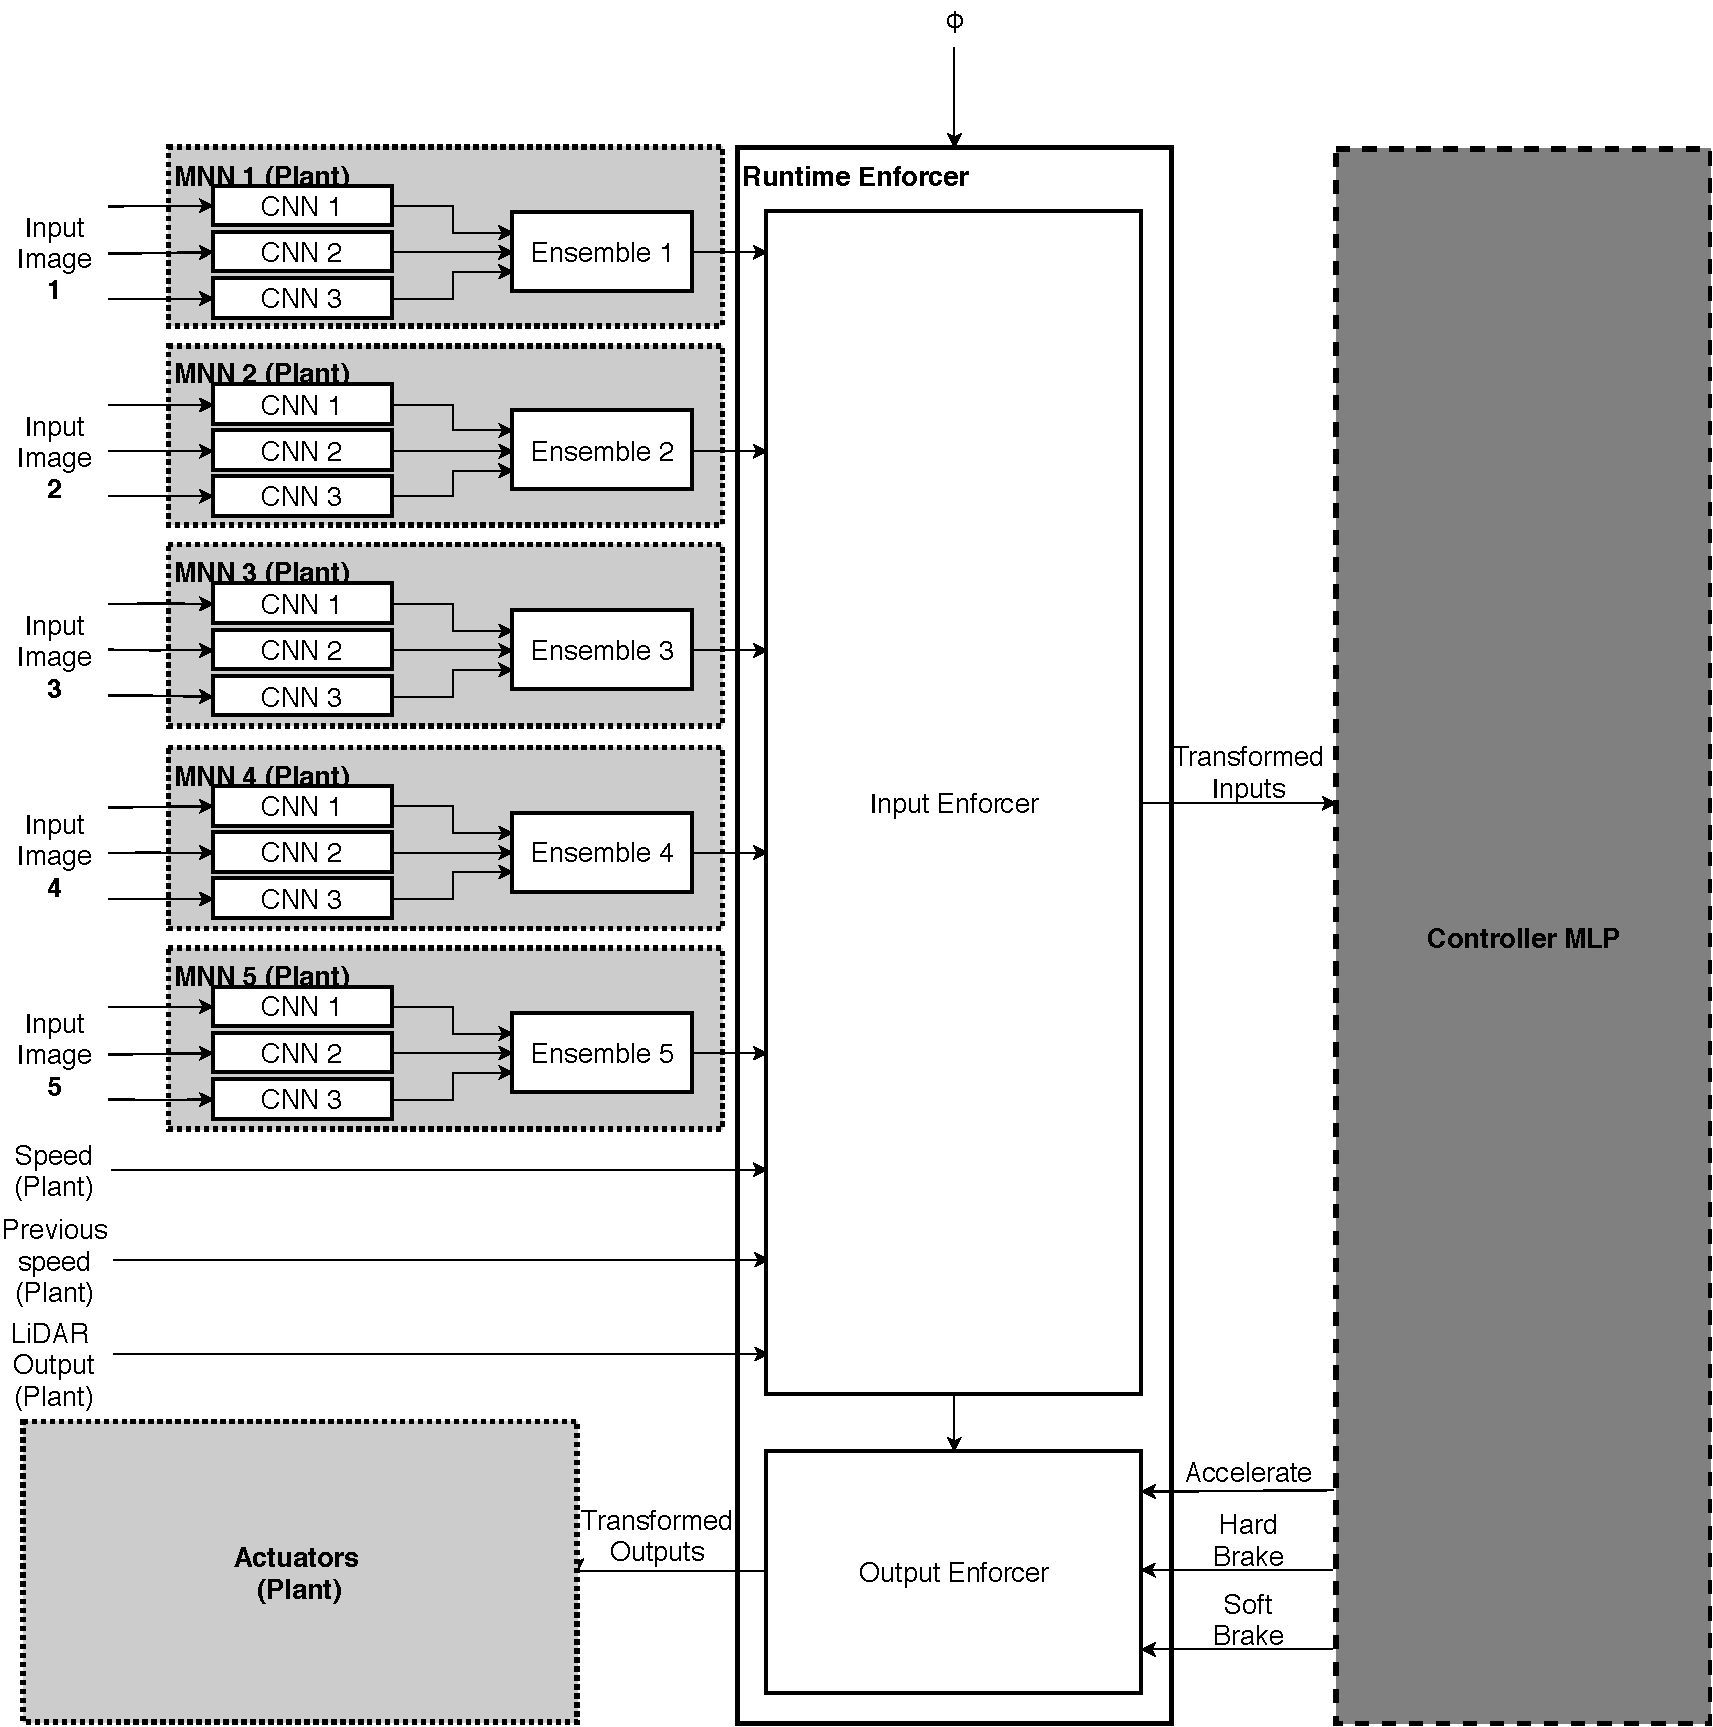
\includegraphics[width=\linewidth]{Content/fig/AV-MNN.pdf}
	\caption{Diagram showing the \ac{SNN} for the \ac{AV}. \label{fig:avmnn}}
\end{figure}










